\section{Parallélisation avec OpenMP}

Dans cette partie nous verrons comment l'utilisation d'OpenMP pour tirer profit de l'architecture multic\oe ur des processeurs permet d'améliorer sensiblement les performances du programme

\subsection{Approche naïve}

Une première étape dans la parallélisation du programme consiste à y insérer des \\
$\# pragma\ omp\ parallel\ for$ afin de paralléliser le parcours des atomes. On obtient ainsi une accélération qui tend vers des valeurs situées entre 3 et 4, ce qui est conforme à ce qu'on s'attend à voir, avec une machine tournant sur un processeur à 4 c\oe urs, en prenant en considération le fait que seul les processus de calculs sont parallélisées et non pas l'intégralité du programme (d'où des valeurs inférieures à 4 seloin la loi d'Amdahl).

\begin{figure}[!h]
    \centering
    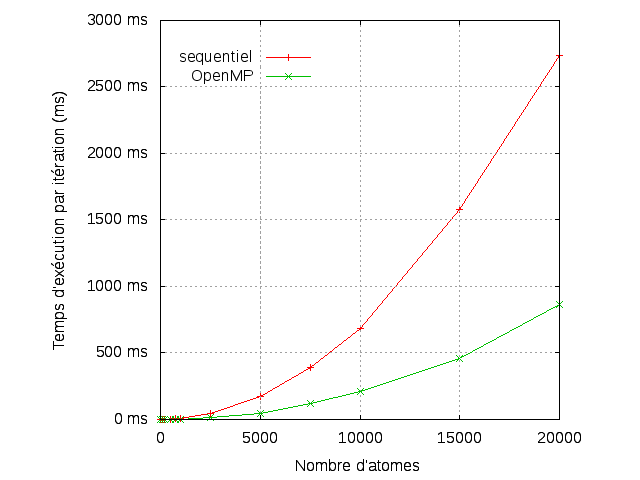
\includegraphics[scale=0.7]{./img/seqomp.png}
    \caption{Comparatif séquentiel/parallèle}
\end{figure}

Toutefois, l'accélération n'est toujours pas suffisante pour pouvoir exécuter une simulation comportant un très grand nombre d'atomes comme $biochoc1$. 
Ceci étant dit, nous pouvons encore améliorer l'algorithme en triant les atomes en fonction de leurs coordonnées, de façon à ne pas parcourir à chaque fois l'intégralité des atomes, ce qui permet de limiter le nombre de calculs (le calcul de la distance étant particulièrement coûteux).  

\subsection{Tri des atomes}
Nous avons vu que le calcul de la force est la partie qui demande le plus de ressources. Ainsi, si nous pouvons éviter des calculs inutiles dans cette partie, les performances du programme n'en seront que meilleures.
Etant donné que nous faisons le choix de négliger la force entre deux atomes lorsque ceux-ci sont éloignés l'un de l'autre d'une distance au moins égale au rayon de coupure. Ainsi, en triant les atomes, nous pouvons faire en sorte de ne parcourir qu'un sous-ensemble restreint d'atomes situés à proximité de l'atome considéré.

\paragraph{Tri par Z}
Dans un premier temps, les atomes sont triés par leurs coordonnées selon Z. Ainsi, lorsque l'on effectue le parcours du tableau d'atomes, nous pouvons nous arrêter dès lors que l'on voit que l'écart sur l'axe Z dépasse le rayon de coupure.
Le tri est effectué selon l'algorithme du tri par tas, dont la complexité est en $O(n log(n))$

Il y a cependant un défaut à ce tri. En effet, il n'est d'aucune aide si tous les atomes sont situés sur un même plan orthogonal à l'axe Z.

\paragraph{Tri par boîtes}
Désormais, l'espace est découpé en petits cubes de taille égale au rayon de coupure. Chaque atome se retrouve alors dans un des cubes de l'espace. Pour chacun d'entre eux, nous pouvons alors ne considérer que les atomes situés dans les 26 cubes situés autour de celui auquel il appartient.
Le processus de tri est toutefois un peu plus élaboré que pour le tri par Z. Pour ce faire, nous avons défini en tant que variables globales, deux tableaux intermédiaires dans lesquels vont être stockés les positions et les vitesses des atomes suivant leur nouvel indice. Nous avons également défini un tableau qui associe à chaque numéro de boîte le nombre d'atomes présents à l'intérieur ainsi qu'un tableau donnant le nouvel indice d'un atome en fonction de son numéro de boîte.

Dans un premier temps, le but est de calculer le nombre d'atomes présents dans chaque boîtes. Ceci se fait aisément en parcourant la table des atomes et en calculant pour chaque atome l'indice de boîte à laquelle ils appartiennent en fonction de leur position dans l'espace.

\begin{table}[!h]
\centering
\begin{minipage}{\linewidth}
\centering
\begin{tabular}{|c|c|c|c|c|c|c|}
  \hline
  Numéro de boite & 0 & 1 & 2 & 3 & ...&  n \\
  \hline
  Nombre d'atomes & 1 & 0 & 15 & 6 & ... & 10 \\
  \hline
\end{tabular}
\end{minipage}

\begin{minipage}{\linewidth}
\centering
\begin{tabular}{|c|c|c|c|c|c|c|}
  \hline
  Numéro de boite & 0 & 1 & 2 & 3 & ... & n \\
  \hline
  Cumulé & 0 & 1 & 1 & 16 & ... & $nb\_atomes[n-1]+cumule[n-1]$ \\
  \hline
\end{tabular}
\end{minipage}
\caption{Tableau supérieur : Nombre d'atomes par boite \\
        Tableau inférieur : Tableau des cumulés associé}
\end{table}

Dans un second temps, une fois le nombre d'atomes par boîte calculé, on remplit un tableau des cumulés (voir la table ci-dessus). Cela nous permet de relier un numéro de boîte d'un atome à son nouvel indice. Nous pouvons désormais copier vers les tableaux intermédiaires, les positions et vitesses des atomes, aux nouveaux indices que nous donne le tableau des cumulés (Dans l'exemple ci-dessus, le premier atome de la boîte 3 rencontrée devra être placé à l'indice 16).

Lorsqu'un atome est placé à son nouvel indice, le tableau des cumulés est incrémenté à la case correspondant à son numéro de boîte. De cette façon lorsqu'on rencontre un autre atome de la même boîte, on pourra lire directement dans cette case l'indice auquel cet autre atome devra être placé.


Une fois tous les atomes déplacés vers leurs nouvelles positions, le contenu des tableaux intermédiaires est recopié vers le tableau global.

Finalement, le calcul des atomes proches se fait aisément, en calculant le numéro des boîtes voisines et en reliant ces numéros aux indices des atomes par le tableau des cumulés 


\paragraph{Résultats}
\begin{figure}[!h]
    \centering
    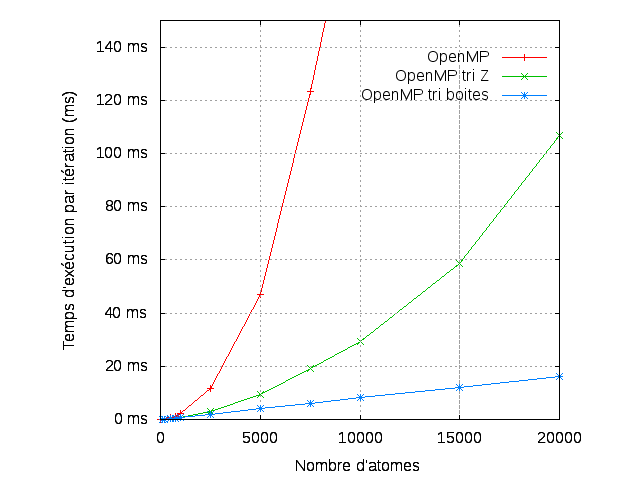
\includegraphics[scale=0.7]{./img/omp3.png}
    \caption{Comparatif OpenMP}
\end{figure}

On peut voir sur ces résultats que le tri par boîtes améliore grandement les performances dans le cas général, notamment lorsque les atomes sont répartis uniformément dans l'espace. Cependant, avec une configuration identique à $3\_atoms\_dim\_400$ où il n'y a que peu d'atomes mais un grand nombre de boîtes, le tri par boîtes se retrouve finalement en-deçà de celui du tri par Z (et même de la version non triée). 
\newpage
A l'inverse, l'algorithme est bien meilleur lorsque les atomes sont tous groupés comme c'est le cas dans la configuration $dense$ (Le calcul est effectué 5 fois plus vite par rapport à la simulation avec l'option $-n\ 1000$, où il y a le même nombre d'atomes mais répartis uniformément dans l'espace).
On remarquera également les faibles résultats obtenus sur $choc2$ avec la version tri par Z qui confirment effectivement l'inefficacité de ce tri lorsque beaucoup d'atomes forment un plan orthogonal à l'axe Z

\begin{table}[!h]
\centering
\begin{tabular}{|l|l|l|l|l|l|}
  \hline
  Fichier & \#atomes & \#boites & Temps/i (\micro s) & Temps/i (\micro s)  \\
  & & & tri par Z & tri par boîtes \\
  \hline
  3\_atoms\_dim\_400 & 3 & 330k & 26 & 3023 \\
  dense & 1000 & 1.3k & 836 & 159 \\
  -n 1000 & 1000 & 1.2k & 783 & 743 \\
  choc2 & 5200 & 176k & 82389 & 6443 \\
  biochoc1 & 40344 & 1.3M & 130399 & 33235 \\
  \hline
\end{tabular}
\caption{Comparaison des tris}
\end{table}


